\subsection{进程切换}
进程切换是操作系统中的一项核心功能,其作用是在多任务操作系统中实现进程间的切换,使得每个进程都可以独立地运行并且感觉到自己在独占CPU。 \\
实现进程的切换具有以下几个重要作用:
\begin{enumerate}
	\item 提高系统的并发性:进程切换可以使得多个进程在同一时刻并发运行,从而提高系统的效率和资源利用率。
	\item 实现多任务操作系统的核心功能:进程切换是多任务操作系统的核心功能之一,它可以使得每个进程都独立运行,并且感觉到自己在独占CPU。
\end{enumerate}
总之,进程切换是操作系统中一项重要的功能,它可以提高系统的并发性和效率,支持多任务和多用户系统,并且是操作系统实现任务调度、资源分配等核心功能的基础。\\

\subsubsection{进程切换的基本流程}
NPUcore进程的切换大致可以分为以下几个步骤:
\begin{enumerate}
	\item 用户态陷入内核态(系统调用或中断)
	\item 切换到调度器进程
	\item 切换到新进程的内核线程
	\item 从内核态返回
\end{enumerate}

\begin{figure}[ht]
	\centering
	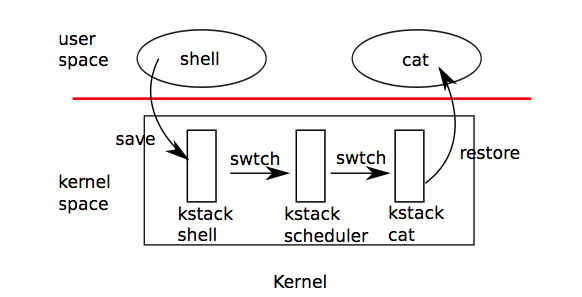
\includegraphics[width=0.8\textwidth]{figures/05-02-03-进程切换.png}
	\caption{进程切换}
\end{figure}



\newpage

为了在进程之间进行切换,NPUcore需要在内核态执行两次上下文切换:从旧进程的内核线程切换到CPU的调度器线程,以及从调度器线程切换到新进程的内核线程。
进程切换的核心\textbf{\_\_switch}并不了解线程,它只是简单地保存和恢复寄存器集合,即上下文。上下文是CPU保存的当前进程执行的状态。
对于RISC-V,进程上下文包括:\textbf{ra}进程的返回地址、\textbf{sp}进程内核栈指针、\textbf{s0-s11}被调用者保存寄存器。\\

\begin{table}[h]
	\centering
	\begin{tabular}{|c|c|c|c|}
		\hline
		\textbf{Register} & \textbf{ABI Name} & \textbf{Description} & \textbf{Saver} \\
		\hline
		x0 & zero & Hard-wired zero & --- \\
		x1 & ra & Return address & Caller \\
		x2 & sp & Stack pointer & Callee \\
		x3 & gp & Global pointer & --- \\
		x4 & tp & Thread pointer & --- \\
		x5-7 & t0-2 & Temporaries & Caller \\
		x8 & s0/fp & Saved register/frame pointer & Callee \\
		x9 & s1 & Saved register & Callee \\
		x10-11 & a0-1 & Function arguments/return values & Caller \\
		x12-17 & a2-7 & Function arguments & Caller \\
		x18-27 & s2-11 & Saved registers & Callee \\
		x28-31 & t3-6 & Temporaries & Caller \\
		f0-7 & ft0-7 & FP temporaries & Caller \\
		f8-9 & fs0-1 & FP saved registers & Callee \\
		f10-11 & fa0-1 & FP arguments/return values & Caller \\
		f12-17 & fa2-7 & FP arguments & Caller \\
		f18-27 & fs2-11 & FP saved registers & Callee \\
		f28-31 & ft8-11 & FP temporaries & Caller \\
		\hline
	\end{tabular}
	\caption{RISC-V calling convention register usage.}
\end{table}

\newpage

\subsubsection{NPUcore实现进程切换的方法}
进程的切换依靠 os/src/task/mod.rs 中的 suspend\_current\_and\_run\_next 函数实现。
该函数的应用主要有如下两个场景:
\begin{itemize}
	\item{应用程序手动使用 sys\_yield 系统调用让出当前进程的占用权。}
	\begin{lstlisting}[language={Rust},caption={syscall yield}]
		pub fn sys_yield() -> isize {
			suspend_current_and_run_next();
			SUCCESS
		}
	\end{lstlisting}
	\item{内核触发定时中断}
	\begin{lstlisting}[language={Rust},caption={Timer Interrupt}]
		Trap::Interrupt(Interrupt::SupervisorTimer) => {
			do_wake_expired();
			set_next_trigger();
			suspend_current_and_run_next();
		}
	\end{lstlisting}
\end{itemize}

NPUcore中,suspend\_current\_and\_run\_next 函数实现如下:
\begin{lstlisting}[language={Rust}, caption={suspend current and run next}]
	pub fn suspend_current_and_run_next() {
		// There must be an application running.
		let task = take_current_task().unwrap();
		
		// ---- hold current PCB lock
		let mut task_inner = task.acquire_inner_lock();
		let task_cx_ptr = &mut task_inner.task_cx as *mut TaskContext;
		// Change status to Ready
		task_inner.task_status = TaskStatus::Ready;
		drop(task_inner);
		// ---- release current PCB lock
		
		// push back to ready queue.
		add_task(task);
		// jump to scheduling cycle
		schedule(task_cx_ptr);
	}
\end{lstlisting}

函数首先获取了一个当前正在执行进程的 PCB ,命名为 task 。然后从刚才得到的 PCB 里面的可变部分(类型为使用 MutexGuard 锁保护住的一个泛型结构体
MutexGuard<TaskControlBlockInner> ),获取当前进程的 task\_cx (类型是一个结构体 TaskContext ,保存着当前进程的上下文信息),然后把他转化成一个可变的裸指针。
再当前进程的状态从“正在运行”改为“就绪”,也就是停止当前进程。接着手动调用 drop 让 task\_inner 的引用计数值减一,并调用了 add\_task 方法将进程加入就绪队列。
最后调用 schedule 函数完成进程的切换。\\

TaskContext 的定义如下。ra 为调用后需要返回位置的pc值,它记录了 \_\_switch 函数返回之后应该跳转到哪里继续执行,从而在任务切换完成并 ret 之后能到正确的位置;
sp 为当前程序用户栈的栈指针;s0~s11 是需要保存的12个寄存器。
\begin{lstlisting}[language={Rust},  caption={TaskContext}]
	pub struct TaskContext {
		ra: usize,
		sp: usize,
		s: [usize; 12],
	}
\end{lstlisting}

add\_task方法是将当前的线程加入到懒分配的全局变量TASK\_MANAGER的就绪队列中。
\begin{lstlisting}[language={Rust},  caption={add task}]
	lazy_static! {
		pub static ref TASK_MANAGER: Mutex<TaskManager> = Mutex::new(TaskManager::new());
	}
	
	pub fn add_task(task: Arc<TaskControlBlock>) {
		TASK_MANAGER.lock().add(task);
	}
	impl TaskManager {
		pub fn add(&mut self, task: Arc<TaskControlBlock>) {
			self.ready_queue.push_back(task);
		}
	}
\end{lstlisting}

schedule 函数负责将当前的进程切换到处理器调度进程(idle task)。
处理器调度进程由懒分配的全局变量PROCESSOR管理,切换过程通过汇编代码\_\_switch实现。
\begin{lstlisting}[language={Rust}, caption={TaskContext}]
	pub struct Processor {
		current: Option<Arc<TaskControlBlock>>,
		idle_task_cx: TaskContext,
	}
	lazy_static! {
		pub static ref PROCESSOR: Mutex<Processor> = Mutex::new(Processor::new());
	}
	pub fn schedule(switched_task_cx_ptr: *mut TaskContext) {
		let idle_task_cx_ptr = PROCESSOR.lock().get_idle_task_cx_ptr();
		unsafe {
			__switch(switched_task_cx_ptr, idle_task_cx_ptr);
		}
	}
\end{lstlisting}

\_\_switch 函数接受两个参数,旧进程的内核栈指针和新进程的内核栈指针。
它将旧进程的上下文(sp,ra,s0-s11)保存到内存中,然后从内存从取出新进程的上下文到CPU的寄存器中。
\begin{lstlisting}[language={riscv}, caption={__switch}]
	.altmacro
	.macro SAVE_SN n
	sd s\n, (\n+2)*8(a0)
	.endm
	.macro LOAD_SN n
	ld s\n, (\n+2)*8(a1)
	.endm
	.section .text
	.globl __switch
	__switch:
	# __switch(
	#     current_task_cx_ptr: *mut TaskContext,
	#     next_task_cx_ptr: *const TaskContext
	# )
	# save kernel stack of current task
	sd sp, 8(a0)
	# save ra & s0~s11 of current execution
	sd ra, 0(a0)
	.set n, 0
	.rept 12
	SAVE_SN %n
	.set n, n + 1
	.endr
	# restore ra & s0~s11 of next execution
	ld ra, 0(a1)
	.set n, 0
	.rept 12
	LOAD_SN %n
	.set n, n + 1
	.endr
	# restore kernel stack of next task
	ld sp, 8(a1)
	ret
\end{lstlisting}